\chapter{Задание}

В лабораторной работе анализируется результат выполнения трех программ. Программы демонстрируют открытие одного и того же файла несколько раз. Реализация, когда файл открывается в одной программе несколько раз выбрана для простоты. Однако, как правило, такая ситуация возможна в системе, когда один и тот же файл несколько раз открывают разные процессы или потоки одного процесса. При выполнении асинхронных процессов такая ситуация является вероятной и ее надо учитывать, чтобы избежать потери данных, получения неверного результата при выводе данных в файл или чтения данных не в той последовательности, в какой предполагалось, и в результате при обработке этих данных получения неверного результата.

Каждую из приведенных программ надо выполнить в многопоточном варианте: в программах создается дополнительный поток, а работа с открываемым файлом выполняется в потоках.

Проанализировать работу приведенных программ и объяснить результаты их работы.

\section*{Структура \_IO\_FILE}

\begin{lstlisting}[language=C]
struct _IO_FILE
{
    int _flags;		/* High-order word is _IO_MAGIC; rest is flags. */

    /* The following pointers correspond to the C++ streambuf protocol. */
    char *_IO_read_ptr;	    /* Current read pointer */
    char *_IO_read_end;	    /* End of get area. */
    char *_IO_read_base;	/* Start of putback+get area. */
    char *_IO_write_base;	/* Start of put area. */
    char *_IO_write_ptr;	/* Current put pointer. */
    char *_IO_write_end;	/* End of put area. */
    char *_IO_buf_base;	    /* Start of reserve area. */
    char *_IO_buf_end;	    /* End of reserve area. */

    /* The following fields are used to support backing up and undo. */
    char *_IO_save_base;    /* Pointer to start of non-current get area. */
    char *_IO_backup_base;  /* Pointer to first valid character of backup area */
    char *_IO_save_end;     /* Pointer to end of non-current get area. */

    struct _IO_marker *_markers;
\end{lstlisting}

\begin{lstlisting}[language=C,firstnumber=21]
    struct _IO_FILE *_chain;

    int _fileno;
    int _flags2;
    __off_t _old_offset; /* This used to be _offset but it's too small.  */
 
    /* 1+column number of pbase(); 0 is unknown. */
    unsigned short _cur_column;
    signed char _vtable_offset;
    char _shortbuf[1];
 
    _IO_lock_t *_lock;
#ifdef _IO_USE_OLD_IO_FILE
};
 
struct _IO_FILE_complete
{
    struct _IO_FILE _file;
#endif
    __off64_t _offset;
    /* Wide character stream stuff.  */
    struct _IO_codecvt *_codecvt;
    struct _IO_wide_data *_wide_data;
    struct _IO_FILE *_freeres_list;
    void *_freeres_buf;
    size_t __pad5;
    int _mode;
    /* Make sure we don't get into trouble again.  */
    char _unused2[15 * sizeof (int) - 4 * sizeof (void *) - sizeof (size_t)];
};
\end{lstlisting}

\chapter{Первая программа}

\begin{lstlisting}[language=C]
/* testCIO.c */
#define _XOPEN_SOURCE 600
#include <unistd.h>
#include <stdio.h>
#include <fcntl.h>
#include <pthread.h>

void* task(void *fd)
{
    FILE *fp = fdopen( *(int *)fd, "r");

    char buffer[20];
    setvbuf(fp, buffer, _IOFBF, sizeof(buffer));

    for (char tmp; fscanf(fp, "%c", &tmp) == 1;)
        printf("%c", tmp);
    printf("\n");

    return NULL;
}

int main(void)
{
    int fd = open("alphabet.txt", O_RDONLY);
    pthread_t tid[2];
    
    if (pthread_create(&tid[0], NULL, task, (void *)&fd) != 0 ||
        pthread_create(&tid[1], NULL, task, (void *)&fd) != 0)
    {
        perror("pthread_create");
        return -1;
    }

    pthread_join(tid[0], NULL);
    pthread_join(tid[1], NULL);

    close(fd);
    return 0;
}    
\end{lstlisting}

\clearpage

\section{Результат работы}

\begin{lstlisting}
$ ./testCIO
Abcdeklmnopqrstuvwxyfzghij        
\end{lstlisting}

\section{Обьяснение}

Системный вызов \texttt{open} создает новый файловый дескриптор для файла, открытого только на чтение. Функция \texttt{open} своим именем возвращает индекс созданного дескриптора в таблице открытых файлов процесса (индекс в массиве \texttt{fd\_array} структуры \texttt{files\_struct}).

Функция \texttt{fdopen} создает структуру \texttt{\_IO\_FILE}, ссылающуюся на созданный ранее дескриптор открытого файла. Таким образом в программе создается 2 структуры \texttt{\_IO\_FILE}, ссылающихся на один дескриптор открытого файла.

\texttt{setbuf} позволяет задать буферы и тип буферизации для структур \texttt{\_IO\_FILE}. Таким образом для каждого из потоков задаем буфер, состоящий из 20 элементов, и буферизацию \texttt{\_IOFBF} (fully buffered).

Пусть первый поток первым начал чтение из файла с помощью библиотечной функции \texttt{fscanf(fp, ...)}. Поскольку \texttt{fscanf} -- функция буферизованного ввода, буфер заполнится первыми 20 символами файла, указатель \texttt{f\_pos} установится на следующий за последним считанным символом символ, после этого начнется считывание символов из буфера.

Если в этот момент первый поток потеряет квант и второй поток начнет выполнение, он также вызовет \texttt{fscanf(fp, ...)}, его буфер заполнится оставшимися в файле символами, \texttt{f\_pos} будет указывать на конец файла.

Таким образом, если процессор будет поочередно выделять квант времени каждому из потоков, алфавит будет выведен в произвольном порядке с учетом того, что первые 20 символов читает первый поток, последующие -- второй.

\clearpage

\section*{Связь структур}

\begin{figure}[ht]
    \centering
    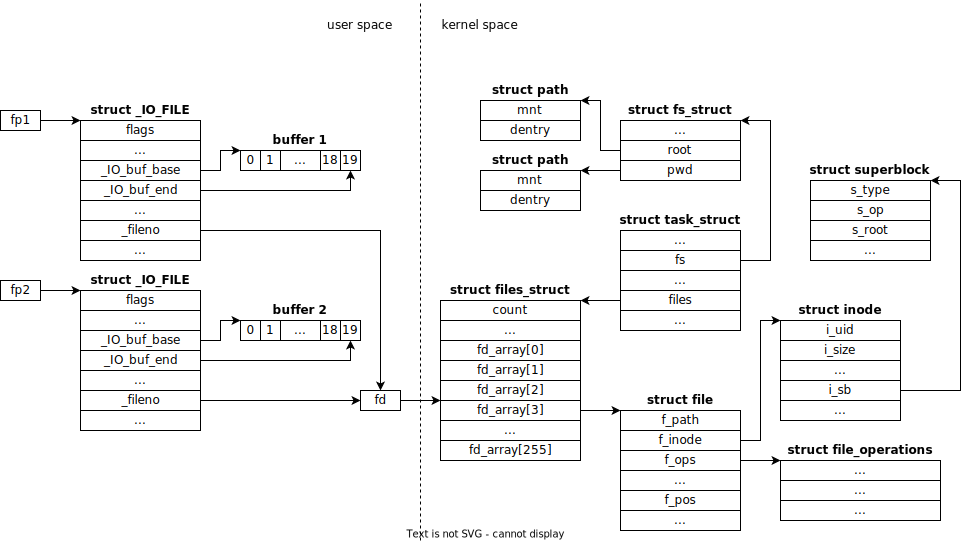
\includegraphics[width=\linewidth]{structs.pdf}
\end{figure}

\chapter{Вторая программа}

\begin{lstlisting}[language=C]
/* testKernelIO.c */
#include <unistd.h>
#include <stdio.h>
#include <fcntl.h>
#include <pthread.h>

void* task(void *data)
{
    int fd = open("alphabet.txt", O_RDONLY);

    for (char c; read(fd, &c, 1) == 1;)
        write(1, &c, 1);

    close(fd);
    return NULL;
}

int main(void)
{
    pthread_t tid1, tid2;
    if (pthread_create(&tid1, NULL, task, NULL) != 0 ||
        pthread_create(&tid2, NULL, task, NULL) != 0)
    {
        perror("pthread_create");
        return -1;
    }

    pthread_join(tid1, NULL);
    pthread_join(tid2, NULL);
    write(1, "\n", 1);
    return 0;
}
\end{lstlisting}

\clearpage

\section{Результат работы}

\begin{lstlisting}
$ ./testKernelIO
AAbcbdcedfegfhgihjikjlkmlnmonpoqprqsrtsutvuwvxwyxzyz
\end{lstlisting}

\section{Объяснение}

Данная программа использует системные вызовы \texttt{read()} и \texttt{write()}, которые не буферизуют ввод/вывод. При каждом вызове \texttt{open()} создается новый дескриптор в таблице открытых файлов процесса, таким образом в каждом из потоков создастся свой дескриптор открытого файла, в связи с чем чтение будет происходить независимо (в каждом из потоков будет изменяться смещение в файле для отдельного дескриптора открытого файла). 

Таким образом, каждый из потоков напечатает по порядку все символы из файла, полученный результат будет зависеть от того, как процессор выделит квант времени потокам.

\clearpage

\section*{Связь структур}

\begin{figure}[ht]
    \centering
    \includegraphics[width=\linewidth]{structs2.pdf}
\end{figure}

\chapter{Третья программа}

\begin{lstlisting}[language=C]
#define _XOPEN_SOURCE 600
#include <stdio.h>
#include <stdlib.h>
#include <pthread.h>
#include <sys/stat.h>

void describe(FILE* fp, const char* prefix)
{
    int pos = ftell(fp);
    struct stat s;
    if (stat("output.txt", &s) != 0)
    {
        perror("stat");
        exit(-1);
    }
    printf("%s: inode = %ld, size = %ld, pos = %d\n", prefix, s.st_ino, s.st_size, pos);
}

void write_syms(FILE* fp, char begin, char end)
{
    while (begin != end)
        fprintf(fp, "%c", begin++);
}

void* task(void* data)
{
    FILE* fp = fopen("output.txt", "wt");
    describe(fp, "fopen");
    char buffer[10];
    setvbuf(fp, buffer, _IOFBF, sizeof(buffer));
    if (data == NULL)
        write_syms(fp, 'a', 'z' + 1);
    else
        write_syms(fp, '0', '9' + 1);
    describe(fp, "fclose");
    fclose(fp);
    return NULL;
}
\end{lstlisting}

\clearpage

\begin{lstlisting}[language=C,firstnumber=39]
int main(void)
{
    pthread_t tid1, tid2;
    if (pthread_create(&tid1, NULL, task, NULL) != 0 ||
        pthread_create(&tid2, NULL, task, (void*)1) != 0)
    {
        perror("pthread_create");
        return -1;
    }

    pthread_join(tid1, NULL);
    pthread_join(tid2, NULL);
    return 0;
}
\end{lstlisting}

\section{Результат работы}

\begin{lstlisting}[language=Bash]
$ ./testFFIO
fopen: inode = 28709680, size = 0, pos = 0
fopen: inode = 28709680, size = 20, pos = 0
fclose: inode = 28709680, size = 20, pos = 10
fclose: inode = 28709680, size = 20, pos = 26
$ cat output.txt
0123456789klmnopqrstuvwxyz
\end{lstlisting}

\section{Объяснение}

В данной программе каждый из потоков открывает один и тот же файл на запись. Поскольку используется функция \texttt{fopen()}, которая создает экземпляр структуры \texttt{\_IO\_FILE}, речь идет о буферизованном выводе. Для каждого из потоков создается свой дескриптор открытого файла в режиме записи. Один поток записывает в файл английский алфавит, другой -- цифры от 0 до 9. Итоговый результат зависит от выделения процессором квантов времени потокам. 

Возможны три ситуации:

\begin{enumerate}
    \item В файле окажутся записаны только цифры. Такой результат говорит о том, что соответствующему потоку был выделен больший квант времени и он успел завершить все операции с файлом до того, как другой поток начал с ним работать, то есть первый вызвал \texttt{fclose()} раньше, чем второй вызвал \texttt{fopen()}.
    
    В таком случае вызов функции \texttt{fopen()} вторым потоком сотрет всю записанную главным потоком информацию, она будет полностью утеряна, второй поток запишет свою информацию, закроет файл, данные запишутся из буфера в файл.

    \item В файле начало алфавита окажется затерто цифрами. Такой результат говорит о том, что оба потока открыли файл на запись до того, как второй вызвал \texttt{fclose()}, и они начали писать в него одновременно. Так как часть символов алфавита затерта цифрами, первый поток вызвал \texttt{fclose()} раньше второго, записав всю информацию из буфера в файл. После этого \texttt{fclose()} вызвал второй поток, записал всю информацию из буфера в файл, чем затер записанную первым потоком информацию.
    \item В файле записан только алфавит. Такой результат может быть следствием двух исходов:
    
    \begin{enumerate}[a)]
        \item Второй поток закончил работу с файлом раньше, чем с ним начал работать первый поток.
        \item Второй поток писал в файл одновременно с первым потоком, но вызвал \texttt{fclose()} раньше, чем первый поток, в связи с чем при вызове \texttt{fclose()} первым потоком информация была полностью затерта.
    \end{enumerate}
\end{enumerate}

Решить перечисленные выше проблемы можно двумя способами:

\begin{enumerate}
    \item Открывать файл в режиме \texttt{O\_APPEND}. В таком случае каждой операции гарантируется неделимость, перед каждым вызовом \texttt{write()} смещение устанавливается в конец файла.
    \item Использовать \texttt{lseek()} и мьютексы для обеспечения монопольного доступа к файлам.
\end{enumerate}

\clearpage

\section*{Связь структур}

\begin{figure}
    \centering
    \includegraphics[width=\linewidth]{structs3.pdf}
\end{figure}

\section*{С использованием блокировок}

\begin{lstlisting}[language=C]
#define _XOPEN_SOURCE 600
#include <stdio.h>
#include <stdlib.h>
#include <pthread.h>
#include <sys/stat.h>

pthread_mutex_t mutex;

void describe(FILE* fp, const char* prefix)
{
    int pos = ftell(fp);
    struct stat s;
    if (stat("output.txt", &s) != 0)
    {
        perror("stat");
        exit(-1);
    }
\end{lstlisting}

\begin{lstlisting}[language=C,firstnumber=18]
    printf("%s: inode = %ld, size = %ld, pos = %d\n", prefix, s.st_ino, s.st_size, pos);
}

void write_syms(FILE* fp, char begin, char end)
{
    pthread_mutex_lock(&mutex);
    fseek(fp, 0, SEEK_END);
    while (begin != end)
        fprintf(fp, "%c", begin++);
    pthread_mutex_unlock(&mutex);
}

void* task(void* data)
{
    FILE* fp = fopen("output.txt", "at");
    describe(fp, "fopen");

    char buffer[10];
    setvbuf(fp, buffer, _IOFBF, sizeof(buffer));

    if (data == NULL)
        write_syms(fp, 'a', 'z' + 1);
    else
        write_syms(fp, '0', '9' + 1);

    describe(fp, "fclose");
    fclose(fp);
    return NULL;
}

int main(void)
{
    pthread_mutex_init(&mutex, NULL);
    pthread_t tid1, tid2;
    if (pthread_create(&tid1, NULL, task, NULL) != 0 ||
        pthread_create(&tid2, NULL, task, (void*)1) != 0)
    {
        perror("pthread_create");
        return -1;
    }

    pthread_join(tid1, NULL);
    pthread_join(tid2, NULL);
    return 0;
}    
\end{lstlisting}

\section*{Результат работы}

\begin{lstlisting}[language=Bash]
$ ./testFFIO && cat output.txt
fopen: inode = 28709680, size = 0, pos = 0
fopen: inode = 28709680, size = 0, pos = 0
fclose: inode = 28709680, size = 0, pos = 10
fclose: inode = 28709680, size = 30, pos = 36
0123456789abcdefghijklmnopqrstuvwxyz    
\end{lstlisting}
